\begin{table*}[t!]
\begin{center}
\begin{tabular}{ccccc}
 &  & \multicolumn{3}{c}{\textsc{Base Visualization}} \\
 &  & \textit{grouped} & \textit{aligned} & \textit{randomized} \\
\multirow{4}{*}{\rotatebox{90}{\textsc{Interaction}}} 
    & \rotatebox{90}{\textit{cbAll} \textbackslash \textit{cbNone}} 
    & 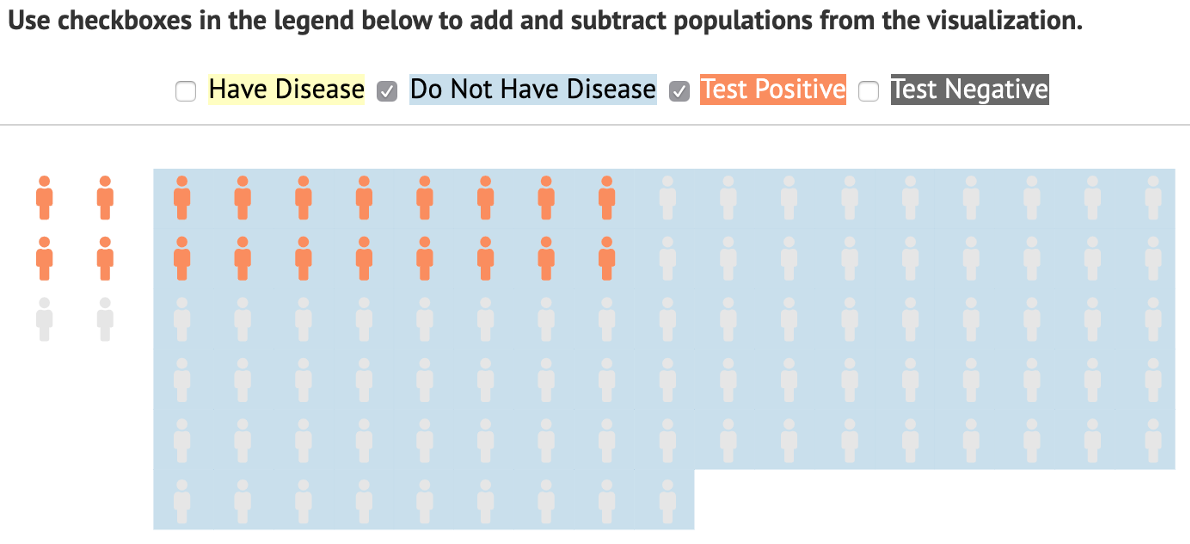
\includegraphics[width=.29\linewidth]{grouped_cbAll.png}  
    & 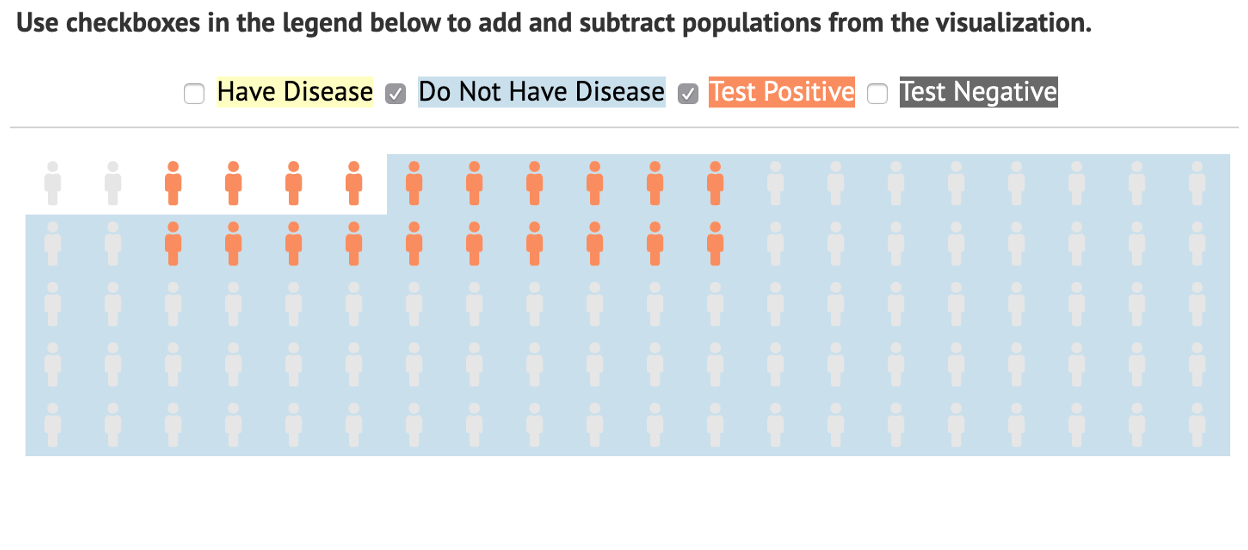
\includegraphics[width=.29\linewidth]{aligned_cbAll.png}  
    & 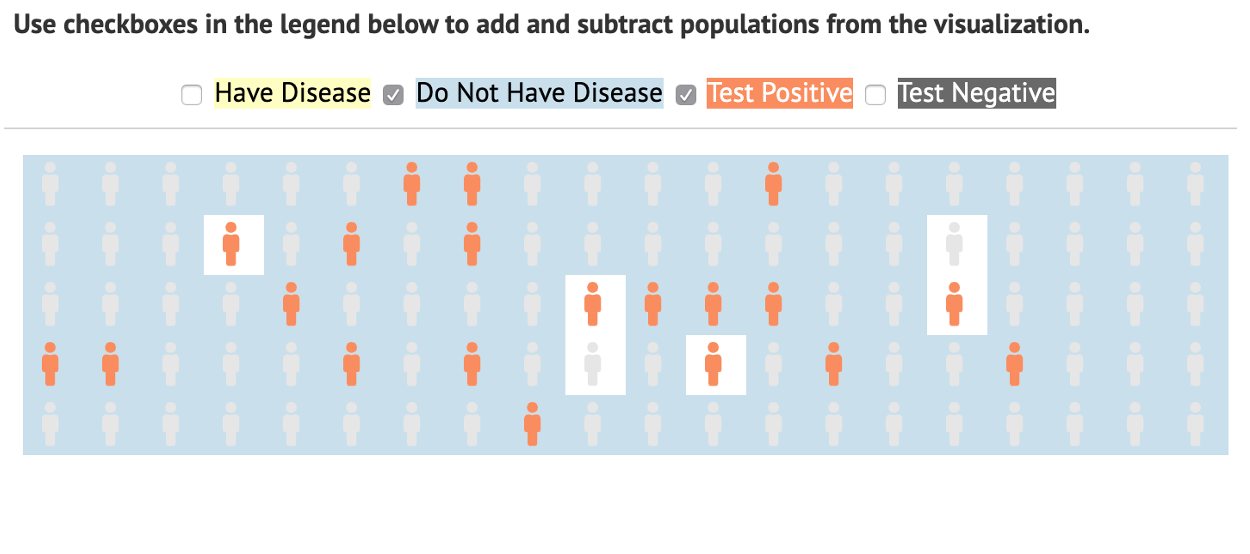
\includegraphics[width=.29\linewidth]{randomized_cbAll.png}
   % \\
   % & \rotatebox{90}{\textit{cbNone}} 
   % & 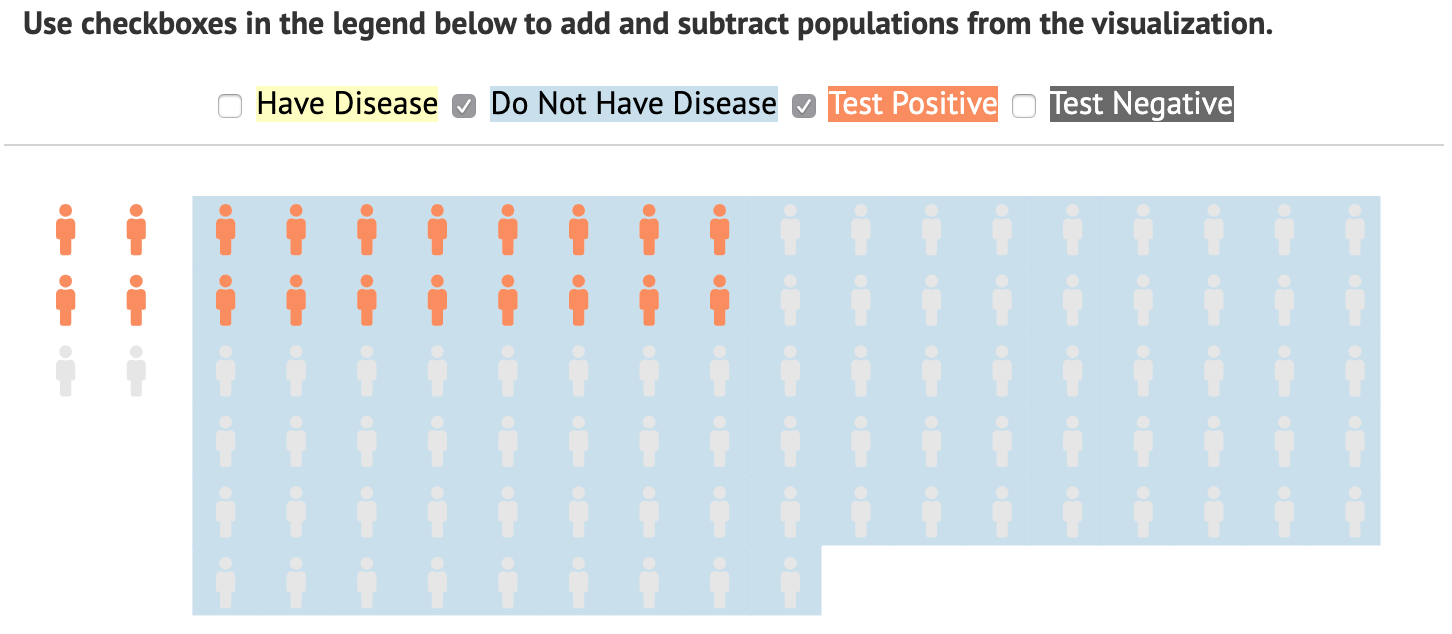
\includegraphics[width=.29\linewidth]{grouped_cbNone.png}  
   % & 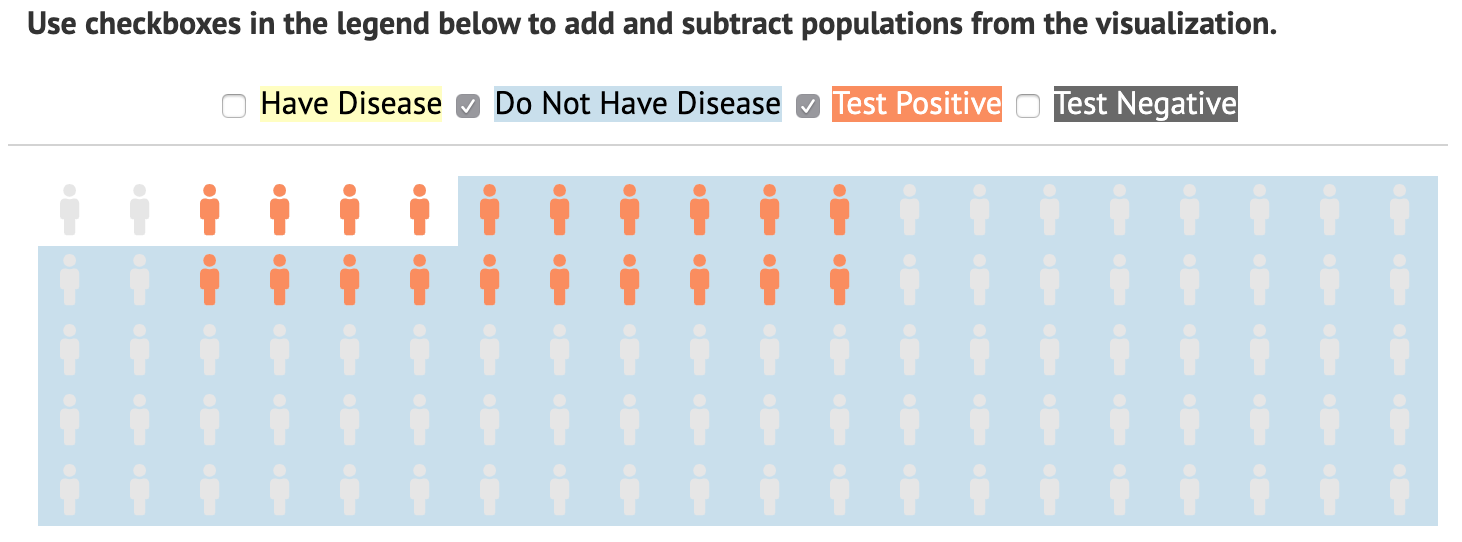
\includegraphics[width=.29\linewidth]{aligned_cbNone.png}  
   % & 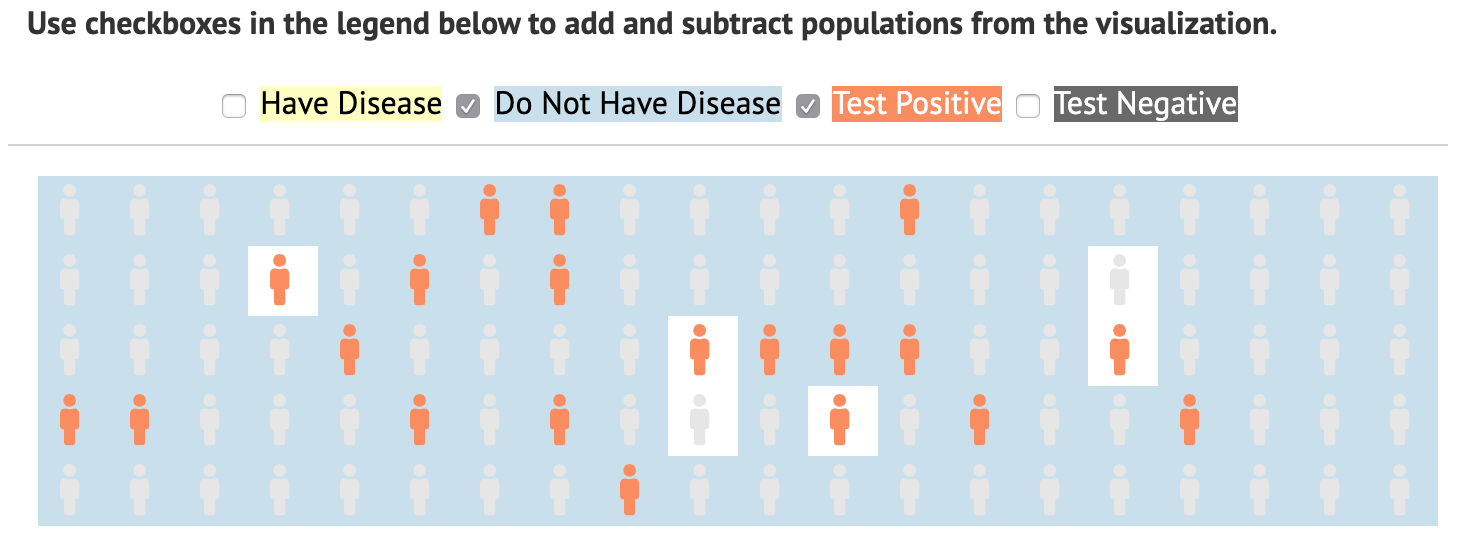
\includegraphics[width=.29\linewidth]{randomized_cbNone.png}
    \\
    & \rotatebox{90}{\textit{drag}} 
    & 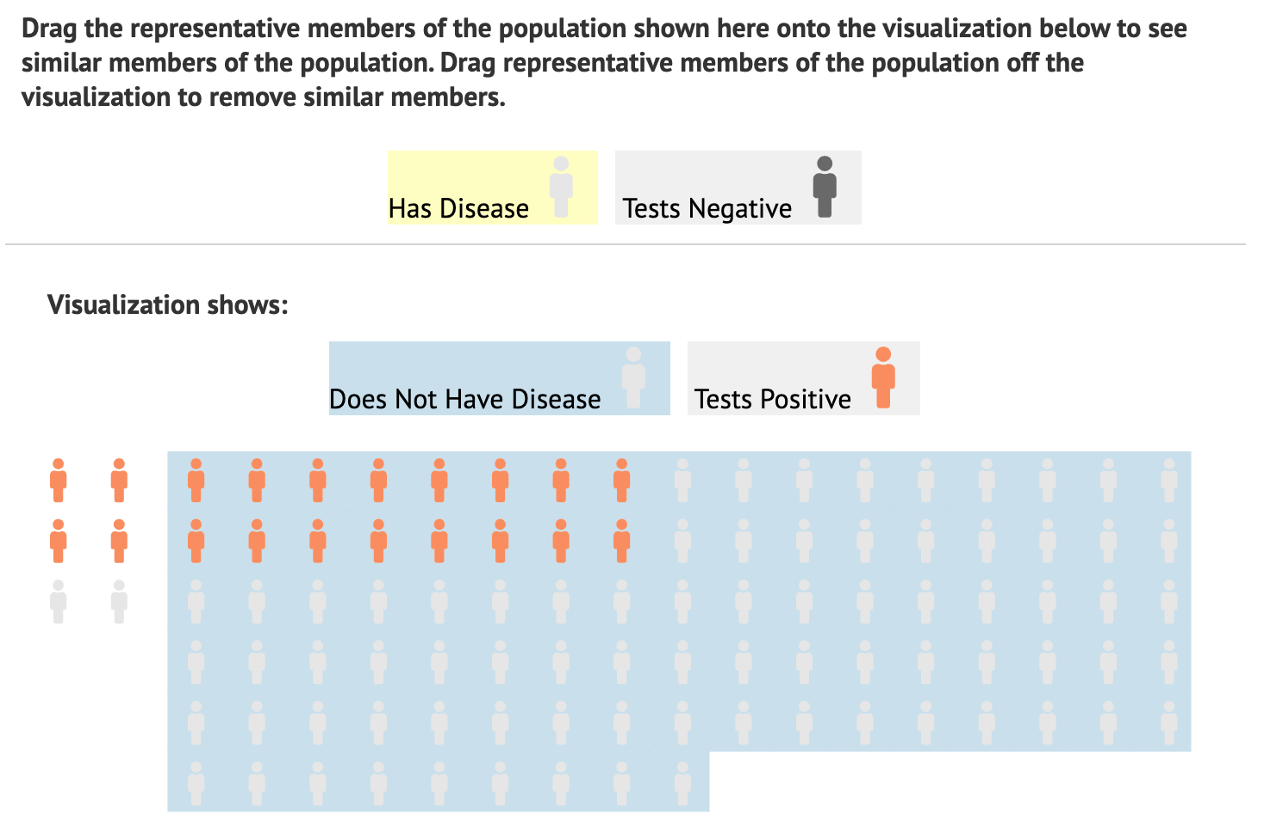
\includegraphics[width=.29\linewidth]{grouped_drag.png}  
    & 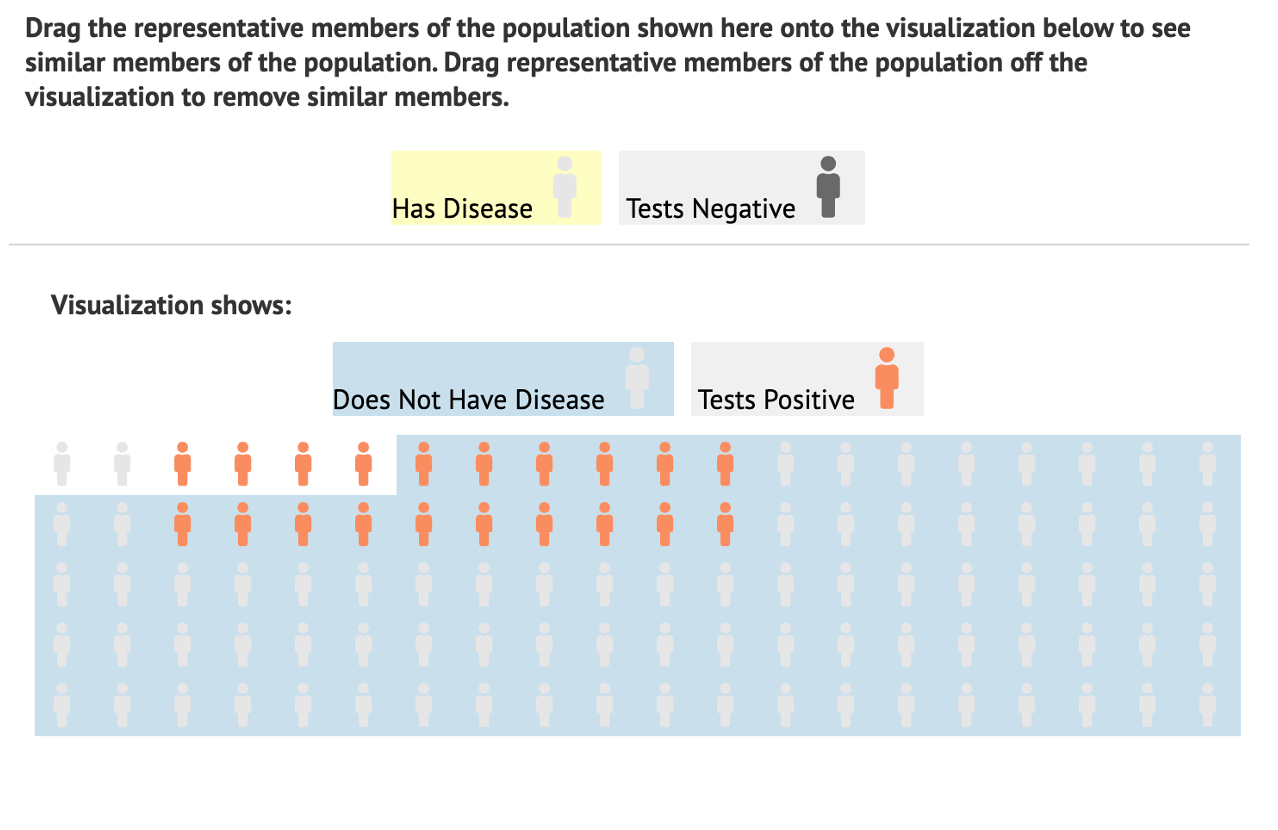
\includegraphics[width=.29\linewidth]{aligned_drag.png}  
    & 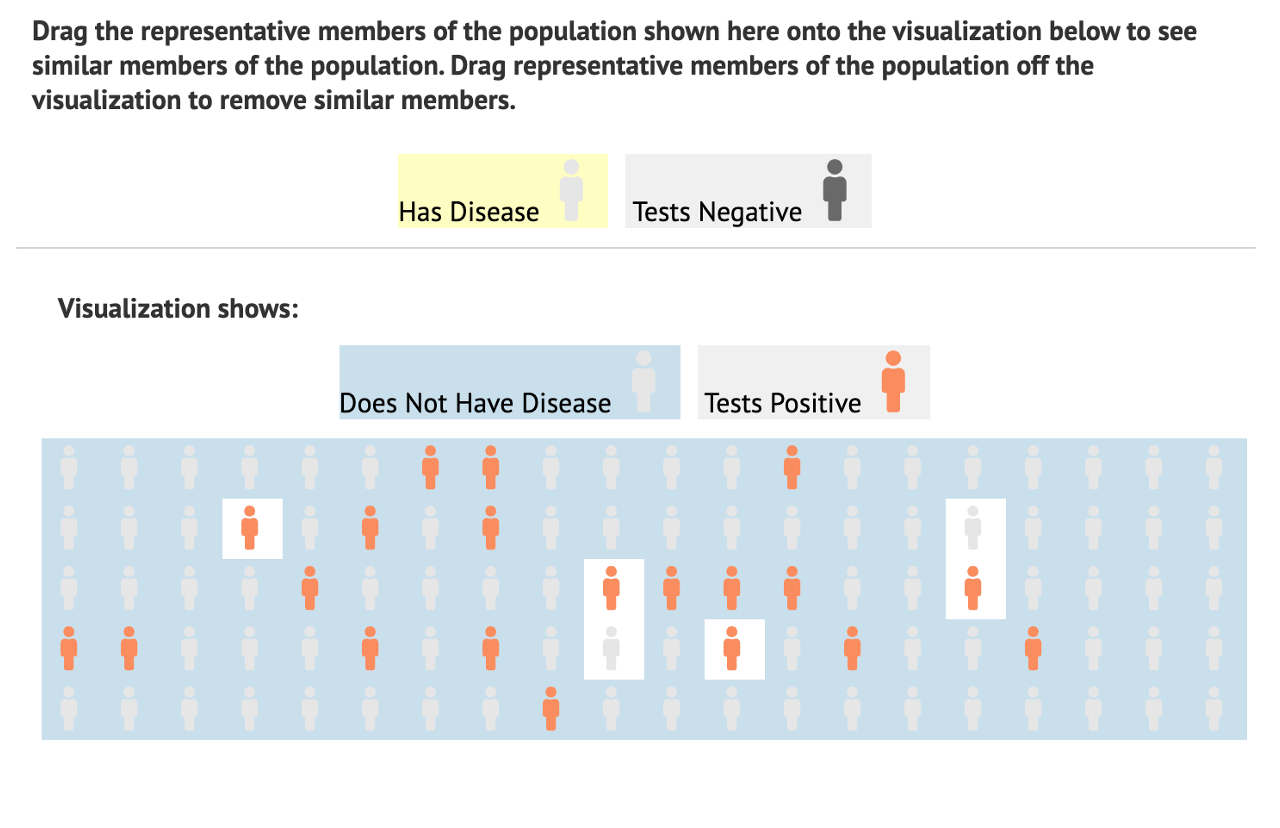
\includegraphics[width=.29\linewidth]{randomized_drag.png}
    \\
    & \rotatebox{90}{\textit{hover}} 
    & 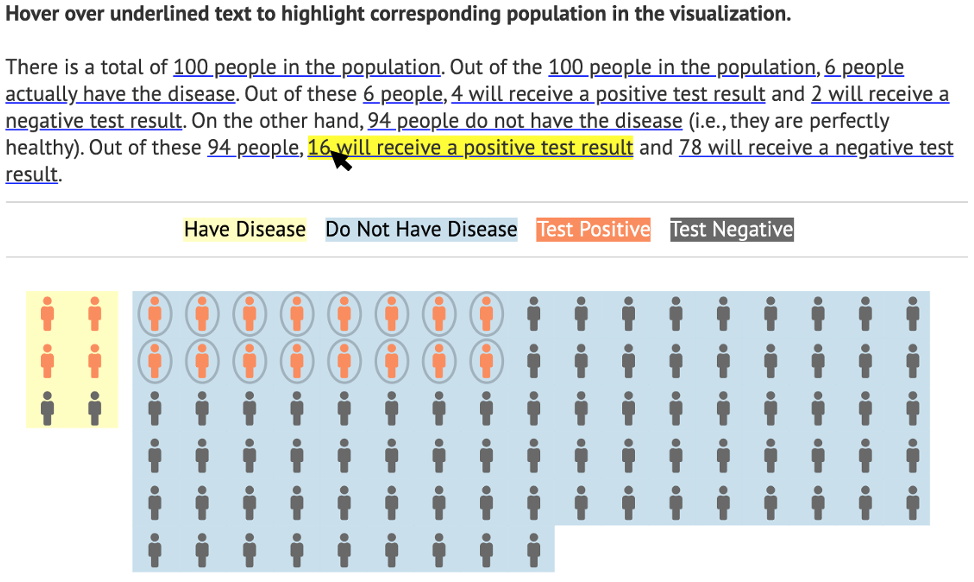
\includegraphics[width=.29\linewidth]{grouped_hover.png}  
    & 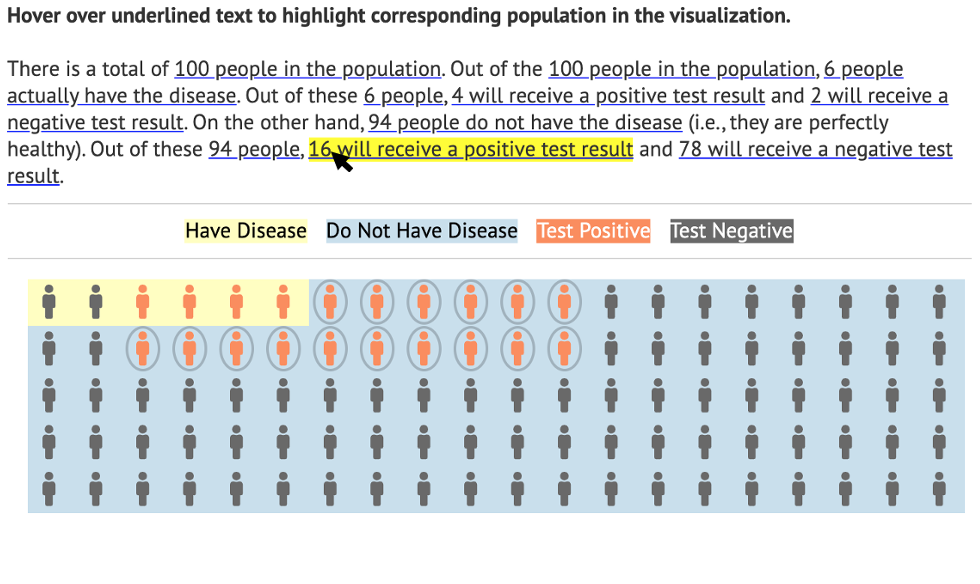
\includegraphics[width=.29\linewidth]{aligned_hover.png}  
    & 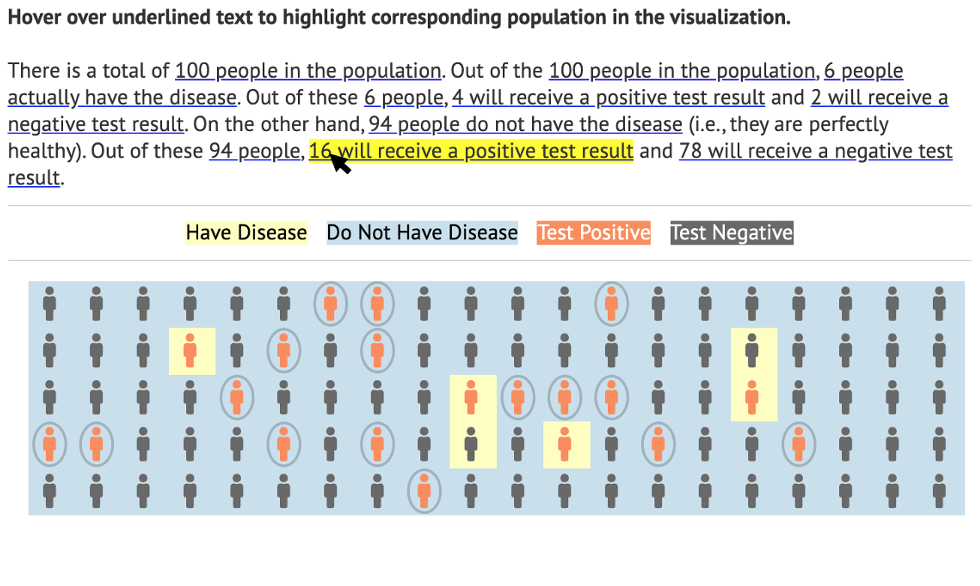
\includegraphics[width=.29\linewidth]{randomized_hover.png}
    \\
    & \rotatebox{90}{\textit{tooltip}} 
    & 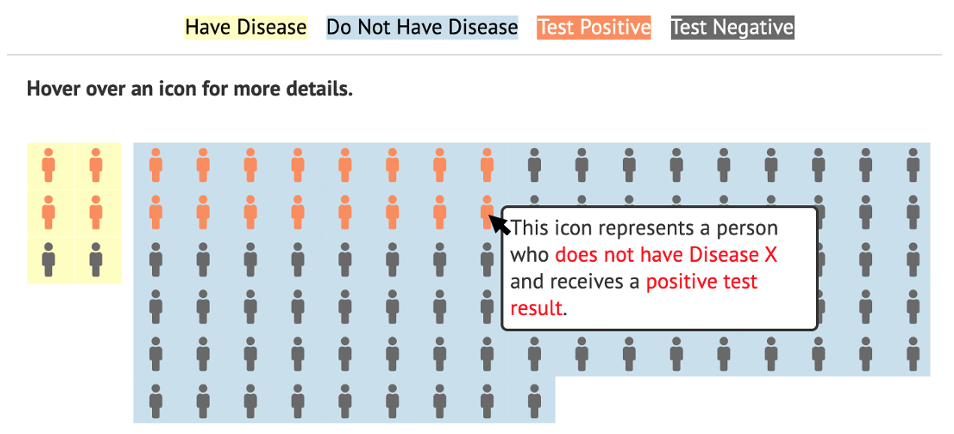
\includegraphics[width=.29\linewidth]{grouped_tooltip.png}  
    & 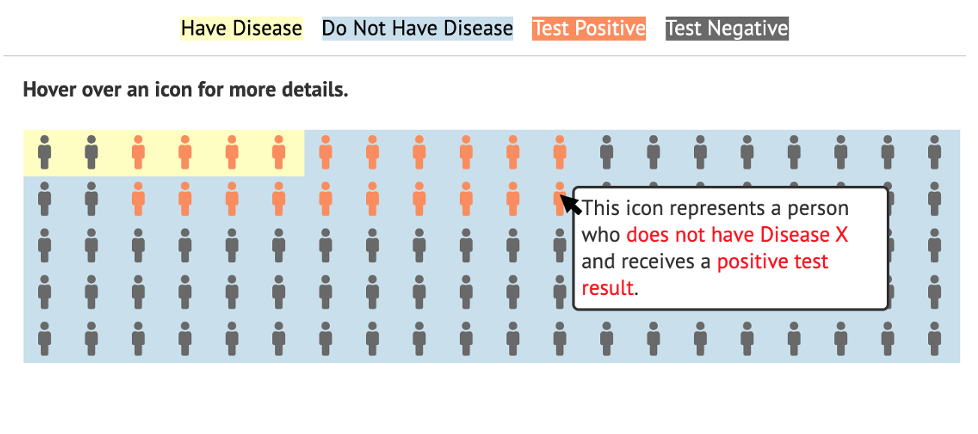
\includegraphics[width=.29\linewidth]{aligned_tooltip.png}  
    & 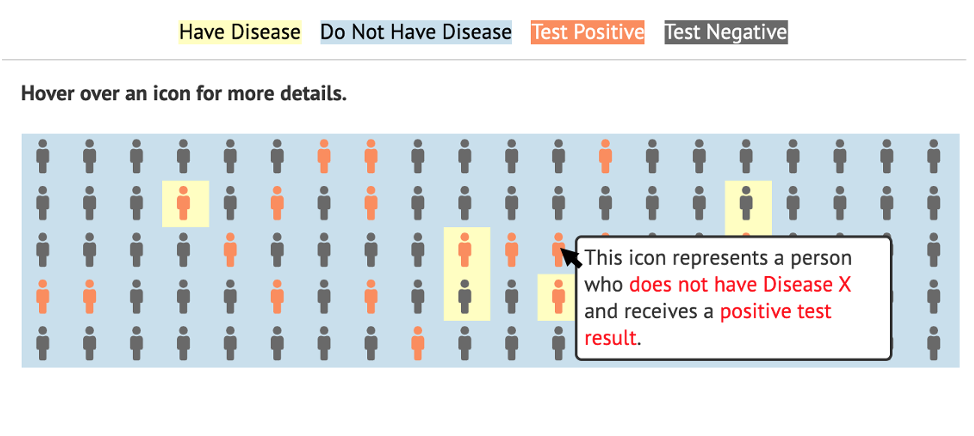
\includegraphics[width=.29\linewidth]{randomized_tooltip.png}
\end{tabular}
\end{center}
\caption{Five interactive conditions used in Experiment 2. Full size images are available in supplementary materials.}
\label{tab:tabFullVis}
\end{table*}


\section{Experiment 2}
The findings of Experiment 1 demonstrated that, depending on the base visualization, adding a \textit{checkbox} interaction to a static Bayesian inference visualization can improve users' reasoning accuracy. Experiment 2 builds on this result by exploring the effect of different interaction designs (\textbf{RQ3}). Specifically, we compare the effects of adding \textit{two types of checkboxes}, \textit{drag and drop}, \textit{brushing and linking}, and \textit{tooltips} to the three \textit{icon array} base visualizations used in Experiment 1. 
In addition to investigating interaction designs, we also examine whether spatial ability moderates the effectiveness of the added interaction (\textbf{RQ4}). Prior work shows that spatial ability plays a significant role in the effective utilization of visualizations~\cite{liu2020Survey}, and in Bayesian reasoning~\cite{ottley2016Bayesian}. Thus we postulate spatial ability can mediate the value-add of interaction to a static Bayesian reasoning visualization. 

\subsection{Visualization Designs}
Consistent with Experiment 1, each stimulus was an icon array that encoded the four key sub-populations in the Bayesian reasoning problem. %: \textsc{Have Disease},  \textsc{Do Not Have Disease}, \textsc{Test Positive}, and  \textsc{Test Negative}. 
Examples of stimuli are shown in Table \ref{tab:tabFullVis}. Experimental factors were:
\begin{itemize}
    \item \textbf{base visualization}: \{\textit{grouped, aligned, randomized}\}
    \item \textbf{interaction technique}: \{\textit{checkboxes (cbAll, cbNone), drag and drop (drag), brushing and linking (hover), tooltips (tooltip)}\}
\end{itemize}

\subsubsection{Base Visualizations}
Experiment 2 used the same three \textit{icon array} base visualizations as Experiment 1 (\textit{grouped}, \textit{aligned}, \textit{randomized}). 

\subsubsection{Interaction Techniques}
We tested five different interaction techniques. Two types of checkboxes were included for consistency with Experiment 1, and because they were tested in prior work on interactive Bayesian reasoning visualizations~\cite{tsai2011Interactive}. Similarly, we included drag and drop as an interaction technique because of its use in prior work on interactive Bayesian reasoning visualizations~\cite{khan2018Interactive}. 
In addition, we tested brushing and linking and tooltips. We included these techniques because they are popular in the visualization community, and are representations of the well known ``\textit{overview first, zoom and filter, details on demand}" mantra of visualization design~\cite{shneiderman1996Eyes}. We chose brushing and linking as an interaction representative of the \textit{zoom and filter} portion of the mantra,
%Moreover, prior work found that people struggle to integrate text and visual representations of the Bayesian reasoning problem\cite{ottley2016Bayesian, ottley2019Curious}. We hypothesize that brushing and linking between text and visualization may overcome this problem. 
and tooltips as an example of the \textit{details on demand} portion of the mantra. Implementation of each technique is explained below:    

\begin{compacthang} 
\item \textbf{\textit{Checkbox All}}: The \textit{cbAll} interaction technique from Experiment 1 was tested in Experiment 2 with a minor modification. Any sub-population checked on the legend is shown on the visualization with color. Any sub-population unchecked on the legend is shown on the visualization with light grey placeholders.      

\item \textbf{\textit{Checkbox None}}: Checkbox None (\textit{cbNone}) is identical to \textit{cbAll}, except all checkboxes are unchecked by default. In other words, the page loads with only light grey placeholders shown on the visualization. 
   
 \item \textbf{\textit{Drag and Drop}}: Drag and drop (\textit{drag}) is a direct manipulation interaction. In practice, \textit{drag} functions identically to \textit{cbNone} expect that participants drag legend labels onto and off of the visualization to show or not show sub-populations.% (as opposed to checking and unchecking checkboxes). 

 \item \textbf{\textit{Brushing and Linking}}:  Brushing and linking (\textit{hover}) is an example of a filter interaction. As participants hover their mouse over areas of text describing sub-populations in the visualization, the text and corresponding sub-population are highlighted. % in the visualization. %\remco{is the reverse true? Does hovering over the visualization highlight text? If so, say that} \ab{no it's not, there is no good mapping in the reverse direction}

\item \textbf{\textit{Tooltip}}: Tooltips (\textit{tooltip}) are an example of details on demand. When a participant hovers their mouse over any icon in the visualization a text box appears describing to which of the four sub-populations that particular icon belongs.  

\end{compacthang}

\subsection{Task}
We ran a between-subjects 5 \{\textit{interaction techniques}\} \textsc{x} 3 \{\textit{base visualizations}\} factor experiment. The same textual description and questions were used as in Experiment 1 (Section \ref{sec:questions}).  

\subsection{Participants}
We recruited 2,149 participants from Amazon Mechanical Turk. Participation was restricted to workers in the United States with an approval rating greater than $90$ percent. Participants were paid a base rate of $\$0.80$ for participation, plus a bonus of $\$0.10$ for every correct answer. 

Before analysis, participants who skipped entire sections of the experiment or did not follow instructions ($N = 35$), participants who self-identified as colorblind ($N = 134$), and participants who saw an interactive visualization but did not interact with it ($N = 473$) were dropped from the data set. 
%\strike{To reiterate, participants who did not interact with a visualization were dropped in order to isolate the effect of \textit{using} interaction from the effect of interaction simply being present in a visualization}.  
There were $N = 1,507$ remaining participants. Demographics of participants are shown in Table \ref{tab:fullDemo}.  

\begin{table}[h!]
\begin{threeparttable}[b]
\begin{tabular}{ll}
\hline
N                                                                                & 1,507                                                                                                                                                    \\ \hline
Age                                                                              & \begin{tabular}[c]{@{}l@{}}18-24: 8.1\%, 25-39: 51.0\%, 40-49: 20.1\%, \\ 50-59: 12.8\%, 60+: 7.7\%\end{tabular}                                     \\ \hline
Gender                                                                           & \begin{tabular}[c]{@{}l@{}}Female: 53.7\%, Male: 45.6\%, \\ Non-Binary: 0.3\%\end{tabular}                                                             \\ \hline
Education                                                                        & \begin{tabular}[c]{@{}l@{}}High School: 28.3\%, Bachelors: 49.1\%, \\ Masters: 14.7\%, PhD: 1.4\%, Other: 5.9\%\end{tabular}                            \\ \hline
\begin{tabular}[c]{@{}l@{}}Expertise with \\ Statistical \\ Visualization\end{tabular}                  & \begin{tabular}[c]{@{}l@{}}Novice: 15.8\%, Low-intermediate: 22.0\%, \\ Intermediate: 38.6\%, \\ High-intermediate: 17.9\%, Expert: 5.0\%\end{tabular} \\ \hline
\begin{tabular}[c]{@{}l@{}}Statistical Training \\ 1 (none) - \\ 5 (highly trained) \end{tabular} & \begin{tabular}[c]{@{}l@{}}1: 30.5\%, 2: 23.6\%, 3: 21.5\%, \\ 4: 15.5\%, 5: 7.4\%\end{tabular}                                                         \\ \hline
\end{tabular}
\end{threeparttable}
\caption{Experiment 2 participant demographics.}
\label{tab:fullDemo}
\end{table}

In order to analyze how the various interaction techniques compared to static we included the \textit{static} group from Experiment 1 as an ``interaction technique" in the analysis of Experiment 2, bringing the total number of participants to $N = 1,733$. From here forward the term ``interaction techniques" refers to \textit{cbAll}, \textit{cbNone}, \textit{drag}, \textit{hover}, \textit{tooltip}, and \textit{static}. Participants were assigned to stimuli as shown in Table \ref{tab:fullN}. 

\begin{table}[h!]
  \resizebox{\linewidth}{!}{
  \centering
\begin{tabular}{c|ccc|c}
        & grouped & aligned & randomized &  interaction technique total\\ \hline
\textit{cbAll}   & 42     & 59     & 64 & 165    \\ \hline
\textit{cbNone}  & 131    & 113    & 117 & 361  \\ \hline
\textit{drag}    & 75     & 79     & 99 &   253  \\ \hline
\textit{hover}   & 109    & 114    & 141 & 364   \\ \hline
\textit{tooltip} & 122    & 132    & 110 & 364 \\ \hline
\textit{static}  & 86    & 70    & 70  &  226 \\ \hline
base total &  565 & 567 & 601 & 1733           
\end{tabular}}
\caption{Sample sizes (N) for each condition in Experiment 2.}
\label{tab:fullN}
\end{table}

\subsection{Procedure}
Experiment 2 followed the same procedure as Experiment 1 with two exceptions. First, there was no instruction page, instead instructions were provided alongside each stimulus. And second, participants were asked to complete a an additional NASA-TLX\cite{NASATLX} survey after the completion of the main study to measure task difficulty.

\subsection{Hypotheses}
Analyses for Experiment 2 focused on answering \textbf{RQ3} and \textbf{RQ4}. We postulate that the conflicting conclusions on whether interactive visualization improves (Tsai et. al~\cite{tsai2011Interactive}) or impedes (Khan et al.~\cite{khan2018Interactive}) Bayesian reasoning may be due to differences in underlying static visualizations, and different interaction designs. Consistent with our findings from Experiment 1, we anticipate that the value-add of interaction will be moderated by base visualization and interaction technique (\textbf{RQ3}). Furthermore, %\replace{it is well established that spatial ability effects visualization usage in general~\cite{liu2020Survey}, and performance on Bayesian inference~\cite{ottley2016Bayesian}. Consistent with prior studies on spatial ability and visualization~\cite{liu2020Survey}, we expect users with high spatial ability to adapt and benefit more from interactivity than users with low spatial ability (\textbf{RQ4})}{
we hypothesize that participants' spatial ability will affect their ability to use the visualization to solve the Bayesian reasoning task. Ottley et al.\cite{ottley2016Bayesian} reported that people with high spatial ability perform Bayesian reasoning significantly better than those with low spatial ability. Additionally, investigations into general visualization usage often show that people with high spatial ability are more adaptable to different visualization designs than people with low spatial ability~\cite{liu2020Survey}. In this experiment, we evaluate whether these trends will hold for the use of interactive Bayesian inference visualizations. Specifically, we propose the following hypotheses:

\begin{compacthang} 
	\item \textbf{H3.1}: Participants' accuracy will differ by interaction technique (\textit{cbAll, cbNone, drag, hover, tooltip, static}). 
	\item \textbf{H3.2}: Participants' accuracy will differ by interaction technique (\textit{cbAll, cbNone, drag, hover, tooltip, static}) and base visualization (\textit{grouped, aligned, randomized}).  
	\item \textbf{H4.1}: Participants with high spatial ability will perform equally well given any interaction technique (\textit{cbAll, cbNone, drag, hover, tooltip, static}). 
	\item \textbf{H4.2}: Participants with low spatial ability will perform differently depending on a visualization's interaction technique (\textit{cbAll, cbNone, drag, hover, tooltip, static}).
	\item \textbf{H4.3}: Participants with high spatial ability will perform equally well given any interaction technique (\textit{cbAll, cbNone, drag, hover, tooltip, static}) and base visualization (\textit{grouped, aligned, randomized}). 
	\item \textbf{H4.4}: Participants with low spatial ability will perform differently depending on a visualization's interaction technique (\textit{cbAll, cbNone, drag, hover, tooltip, static})  and base visualization (\textit{grouped, aligned, randomized}).
	
	%\remco{not sure if we should separate this into 4.1 and 4.2 because these two hypotheses are quite nuanced... Without some explanation and background, it could be hard for a reader to understand why we would hypothesize differently for high SA verus low SA participants}
\end{compacthang}

\subsection{Findings}
For each of these hypotheses we performed chi-squared tests to check for significant differences in proportions of correct answers (accuracy). As with Experiment 1, participants were considered correct only if they answered both parts of the two-part question correctly. 

\begin{figure}[h!]
    \centering
    \scalebox{0.7}{
    \begin{bchart}[step=.25,max=1,width=\linewidth]
    \bcbar[label=\textit{cbAll}, color=bar-blue]{.62}
    \bcskip{3pt}
    \bcbar[label=\textit{cbNone}, color=bar-blue]{.58}
    \bcskip{3pt}
    \bcbar[label=\textit{drag}, color=bar-blue]{.57}
    \bcskip{3pt}
    \bcbar[label=\textit{hover}, color=bar-blue]{.48}
    \bcskip{3pt}
    \bcbar[label=\textit{tooltip}, color=bar-blue]{.53}
    \bcskip{3pt}
    \bcbar[label=\textit{static}, color=bar-blue]{.57}
    \bcxlabel{Proportion of Correct Answers}
    \end{bchart}}
    \caption{Portion of participants answering the Bayesian reasoning task correctly given each interaction technique.} %There is a significant pairwise difference between \textit{cbAll} and \textit{hover} ($\chi^2(1, N = 529) = 8.59, p = 0.003$).}
    \label{fig:exp2_interactions}
\end{figure}

\subsubsection{Do different interaction techniques have different effects on accuracy in Bayesian reasoning?} 
We performed a chi-squared test of $accuracy \sim interaction\_technique$, and found a statistically significant difference in accuracy between participants using different interaction techniques ($\chi^2(5, N = 1733 ) = 12.34, p < 0.05$). Pairwise chi-squared tests of interaction techniques with a Bonferroni corrected alpha ($\alpha=0.003$) showed a significant difference between \textit{cbAll} and \textit{hover} ($\chi^2(1, N = 529) = 8.59, p = 0.003$). As shown in Figure \ref{fig:exp2_interactions}, a higher proportion of participants answered the Bayesian reasoning task correctly with the \textit{cbAll} visualization than with the \textit{hover} visualization. These results suggest that \textit{the design of an interactive technique affects the value-add of interaction}, thus we \textbf{accept H3.1}. % depends on design different interaction techniques 
%\remco{Bonferonni correction is very aggressive / conservative, but it's the right thing to do here. The question is, if space permits, would it make sense to list all the p-values? This could give the reader a sense of what the differences are like without the constraint of a very small alpha.}

\begin{figure}[h!]
    \centering
    \scalebox{0.7}{
    \begin{bchart}[step=.25,max=1,width=\linewidth]
    \bcbar[label=\textit{grouped}, color=bar-blue]{.57}
    \bcskip{3pt}
    \bcbar[label=\textit{aligned}, color=bar-blue]{.56}
    \bcskip{3pt}
    \bcbar[label=\textit{randomized}, color=bar-blue]{.52}
    \bcxlabel{Proportion of Correct Answers}
    \end{bchart}}
    \caption{Portion of participants answering the Bayesian reasoning task correctly by base visualization.}
    \label{fig:exp2_bases}
\end{figure}

\subsubsection{Is the effect of interaction moderated by interaction design and the underlying static visualization design?}
We compared participants' accuracy across base visualizations with a chi-squared test of $accuracy \sim base\_visualization$. We found no significant difference in accuracy by base ($\chi^2(2, N = 1733) = 2.98, p = 0.23$), suggesting that \textit{design of the underlying static visualization has no effect on participants' accuracy in a Bayesian reasoning task}. Figure \ref{fig:exp2_bases} shows proportions of correct answers by base visualization. 

\begin{figure}[h!]
    \centering
    \scalebox{0.7}{
    \begin{bchart}[step=.25,max=1,width=\linewidth]
    \bcbar[text=\textit{cbAll},  color=bar-cball]{.74}
    \bcbar[text=\textit{cbNone}, color=bar-cbnone]{.59}
    \bcbar[text=\textit{drag},   color=bar-drag]{.60}
    \bclabel{\textit{grouped}}
    \bcbar[text=\textit{hover},   color=bar-hover]{.51}
    \bcbar[text=\textit{tooltip}, color=bar-tooltip]{.52}
    \bcbar[text=\textit{static},  color=bar-static]{.58}
    \bcskip{6pt}
    
    \bcbar[text=\textit{cbAll},  color=bar-cball]{.61}
    \bcbar[text=\textit{cbNone}, color=bar-cbnone]{.65}
    \bcbar[text=\textit{drag},   color=bar-drag]{.51}
    \bclabel{\textit{aligned}}
    \bcbar[text=\textit{hover},   color=bar-hover]{.48}
    \bcbar[text=\textit{tooltip}, color=bar-tooltip]{.55}
    \bcbar[text=\textit{static},  color=bar-static]{.54}
    \bcskip{6pt}
    
    \bcbar[text=\textit{cbAll},  color=bar-cball]{.55}
    \bcbar[text=\textit{cbNone}, color=bar-cbnone]{.50}
    \bcbar[text=\textit{drag},   color=bar-drag]{.60}
    \bclabel{\textit{randomized}}
    \bcbar[text=\textit{hover},   color=bar-hover]{.45}
    \bcbar[text=\textit{tooltip}, color=bar-tooltip]{.52}
    \bcbar[text=\textit{static},  color=bar-static]{.59}
    
    \bcxlabel{Proportion of Correct Answers}
    \end{bchart}}
    \caption{Portion of participants answering the Bayesian reasoning task correctly given each interaction technique by base visualization.}
    \label{fig:exp2_interactions_by_base}
\end{figure}

Similar to Experiment 1, we stratified data by base visualization (grouped, aligned, randomized) and performed a chi-squared test of $accuracy \sim interaction\_technique$ within each base. Proportions of correct answers by base visualization and interaction technique are shown in Figure \ref{fig:exp2_interactions_by_base}. We found no significant differences in accuracy between participants assigned different interaction techniques within each base (grouped: ($\chi^2(5, N = 565) = 7.77, p = 0.17$), aligned: ($\chi^2(5, N = 567) = 7.75, p = 0.17$), randomized:($\chi^2(5, N = 601) = 6.42, p = 0.27$)), suggesting that \textit{the combination of interaction technique and underlying base visualization has no effect on participants' accuracy in a Bayesian reasoning task}, and causing us to \textbf{reject H3.2} %\remco{Ahhh, this is so confusing and weird! Is H3 about how how different interaction techniques improve reasoning? Or is it about how different interaction techniques, when used with different visualization types, produce different outcomes?}.


\subsubsection{Does the effect of different interaction techniques change based on a user's spatial ability?}
To identify participants with high versus low spatial ability we split our data across median spatial ability ($6.5$), similar to~\cite{ottley2016Bayesian}. We performed a chi-squared test of $accuracy \sim interaction\_technique$ within each spatial ability group. Figure \ref{fig:exp2_sa_by_interaction} shows proportions of correct answers by interaction technique and participants' spatial ability.  

\paragraph{High Spatial Ability}
Within the high spatial ability group we found a statistically significant difference in accuracy between participants using different interaction techniques ($\chi^2(5, N =  881) = 17.70, p < 0.01$). Pairwise chi-squared tests with a Bonferroni corrected alpha ($0.003$) showed a significant difference between \textit{hover} and \textit{static} ($\chi^2(1, N = 287) = 13.60, p < 0.001$). Specifically, a larger proportion of participants answered the Bayesian reasoning task correctly using the \textit{static} visualization versus the \textit{hover} visualization. This suggests that \textit{for people with high spatial ability interaction technique can significantly affect accuracy on Bayesian inference}, thus we \textbf{reject H4.1}. 

\paragraph{Low Spatial Ability}
Within the low spatial ability group we found no statistically significant difference in accuracy between participants using different interaction techniques ($\chi^2(5, N =  852) = 4.46, p = 0.49$), suggesting that \textit{for people with low spatial ability interaction technique does not affect accuracy on Bayesian inference}, thus we \textbf{reject H4.2}. %\remco{this is a little tricky... without careful reading, the rejection of H4.1 and H4.2 makes it feel as if there's no effect of SA on interaction}

\begin{figure}[h!]
    \centering
    \scalebox{0.7}{
    \begin{bchart}[step=.25,max=1,width=\linewidth]
    
    \bcbar[text=\textit{High SA},   color=bar-highsa]{.77}
    \bclabel{\textit{cbAll}}
    \bcbar[text=\textit{Low SA},   color=bar-lowsa]{.43}
    \bcskip{6pt}
    
    \bcbar[text=\textit{High SA},   color=bar-highsa]{.75}
    \bclabel{\textit{cbNone}}
    \bcbar[text=\textit{Low SA},   color=bar-lowsa]{.40}
    \bcskip{6pt}
    
    \bcbar[text=\textit{High SA},   color=bar-highsa]{.69}
    \bclabel{\textit{drag}}
    \bcbar[text=\textit{Low SA},   color=bar-lowsa]{.42}
    \bcskip{6pt}
    
    \bcbar[text=\textit{High SA},   color=bar-highsa]{.62}
    \bclabel{\textit{hover}}
    \bcbar[text=\textit{Low SA},   color=bar-lowsa]{.34}
    \bcskip{6pt}
    
    \bcbar[text=\textit{High SA},   color=bar-highsa]{.71}
    \bclabel{\textit{tooltip}}
    \bcbar[text=\textit{Low SA},   color=bar-lowsa]{.35}
    \bcskip{6pt}
    
    \bcbar[text=\textit{High SA},   color=bar-highsa]{.83}
    \bclabel{\textit{static}}
    \bcbar[text=\textit{Low SA},   color=bar-lowsa]{.35}
    
    \bcxlabel{Proportion of Correct Answers}
    \end{bchart}}
    \caption{Portion of participants answering the Bayesian reasoning task correctly by spatial ability (SA) and interaction technique. } %There is a significant pairwise difference in accuracy between people with high spatial ability in the \textit{hover} and \textit{static} conditions ($\chi^2(1, N = 287) = 13.60, p < 0.001$). Additionally we note participants with high spatial ability perform worse when using an interactive versus static visualization. While participants with low spatial ability perform better using an interactive versus static visualization.}
    \label{fig:exp2_sa_by_interaction}
\end{figure}

%\subsubsection{Does the effect of interaction given different interaction techniques and underlying static visualization designs differ by user's spatial ability?}
\subsubsection{Does underlying static visualization design moderate the effect of interaction techniques within spatial ability groups?}

Within each spatial ability group we compared participants' accuracy across bases with a chi-squared test of $accuracy \sim base\_visualization$. Figure \ref{fig:exp2_bases_by_sa} shows proportions of correct answers for each base visualization by participants' spatial ability. Within both groups we found no significant difference in accuracy by base (high spatial ability: ($\chi^2(2, N = 881) = 1.59, p = 0.45$), low spatial ability: ($\chi^2(2, N = 852) = 5.75, p = 0.06$)), suggesting that \textit{for people with high or low spatial ability, performance on a Bayesian reasoning task is not affected by design of the underlying static visualization}. %\remco{p of 0.06 is pretty close...}

\begin{figure}[h]
    \centering
    \scalebox{0.7}{
    \begin{bchart}[step=.25,max=1,width=\linewidth]
    
    \bcbar[text=\textit{High SA},   color=bar-highsa]{.74}
    \bclabel{\textit{grouped}}
    \bcbar[text=\textit{Low SA},   color=bar-lowsa]{.41}
    \bcskip{6pt}
    
    \bcbar[text=\textit{High SA},   color=bar-highsa]{.72}
    \bclabel{\textit{aligned}}
    \bcbar[text=\textit{Low SA},   color=bar-lowsa]{.40}
    \bcskip{6pt}
    
    \bcbar[text=\textit{High SA},   color=bar-highsa]{.70}
    \bclabel{\textit{randomized}}
    \bcbar[text=\textit{Low SA},   color=bar-lowsa]{.32}

    \bcxlabel{Proportion of Correct Answers}
    \end{bchart}}
    \caption{Proportion of participants answering the Bayesian reasoning task correctly by base visualization for each spatial ability group.}
    \label{fig:exp2_bases_by_sa}
\end{figure}

To investigate the effect of interaction technique coupled with underlying static visualization design on participants with high and low spatial ability, we stratified the data by spatial ability group (high, low) and base visualization (grouped, aligned, randomized) and performed a chi-squared test of $accuracy \sim interaction\_technique$.
Proportions of correct answers by interaction technique, base visualization, and spatial ability are shown in Figure \ref{fig:exp2_corr_by_int_base_SA}. 
Within each spatial ability group and each base visualization we found no significant difference in participants' accuracy between interaction techniques (high spatial ability--grouped: ($\chi^2(5, N = 275) = 8.10, p = 0.15$), aligned: ($\chi^2(5, N = 281) = 7.08, p = 0.22$), randomized:($\chi^2(5, N = 325) = 8.03, p = 0.15$); low spatial ability--grouped: ($\chi^2(5, N = 290) = 3.62, p = 0.61$), aligned: ($\chi^2(5, N = 286) = 6.70, p = 0.24$), randomized:($\chi^2(5, N = 276) = 5.47, p = 0.36$)). These results suggest that \textit{for people with high or low spatial ability the value-add of interaction is not modulated by underlying static visualization design and interaction technique}, thus we \textbf{accept H4.3}, and \textbf{reject H4.4}.  

\begin{figure}[h!]
    \begin{subfigure}[t]{0.52\columnwidth}
    \scalebox{0.7}{
    \begin{bchart}[step=.25,max=1,width=\linewidth]
    \bcbar[text=\textit{cbAll},  color=bar-cball]{.59}
    \bcbar[text=\textit{cbNone}, color=bar-cbnone]{.44}
    \bcbar[text=\textit{drag},   color=bar-drag]{.40}
    \bclabel{\textit{grouped}}
    \bcbar[text=\textit{hover},   color=bar-hover]{.42}
    \bcbar[text=\textit{tooltip}, color=bar-tooltip]{.35}
    \bcbar[text=\textit{static},  color=bar-static]{.38}
    \bcskip{6pt}
    
    \bcbar[text=\textit{cbAll},  color=bar-cball]{.45}
    \bcbar[text=\textit{cbNone}, color=bar-cbnone]{.51}
    \bcbar[text=\textit{drag},   color=bar-drag]{.39}
    \bclabel{\textit{aligned}}
    \bcbar[text=\textit{hover},   color=bar-hover]{.28}
    \bcbar[text=\textit{tooltip}, color=bar-tooltip]{.40}
    \bcbar[text=\textit{static},  color=bar-static]{.36}
    \bcskip{6pt}
    
    \bcbar[text=\textit{cbAll},  color=bar-cball]{.29}
    \bcbar[text=\textit{cbNone}, color=bar-cbnone]{.27}
    \bcbar[text=\textit{drag},   color=bar-drag]{.46}
    \bclabel{\textit{randomized}}
    \bcbar[text=\textit{hover},   color=bar-hover]{.33}
    \bcbar[text=\textit{tooltip}, color=bar-tooltip]{.29}
    \bcbar[text=\textit{static},  color=bar-static]{.27}
    
    \bcxlabel{Proportion of Correct Answers}
    \end{bchart}}
    \caption{\textbf{Low spatial ability}}
    \label{fig:exp2_corr_by_int_base_SA_low}
    \end{subfigure}%
    ~ 
    \begin{subfigure}[t]{0.48\columnwidth}
    \scalebox{0.7}{
    \begin{bchart}[step=.25,max=1,width=\linewidth]
    \bcbar[text=\textit{cbAll},  color=bar-cball]{.84}
    \bcbar[text=\textit{cbNone}, color=bar-cbnone]{.75}
    \bcbar[text=\textit{drag},   color=bar-drag]{.78}
    \bcbar[text=\textit{hover},   color=bar-hover]{.61}
    \bcbar[text=\textit{tooltip}, color=bar-tooltip]{.74}
    \bcbar[text=\textit{static},  color=bar-static]{.82}
    \bcskip{6pt}
    
    \bcbar[text=\textit{cbAll},  color=bar-cball]{.81}
    \bcbar[text=\textit{cbNone}, color=bar-cbnone]{.77}
    \bcbar[text=\textit{drag},   color=bar-drag]{.60}
    \bcbar[text=\textit{hover},   color=bar-hover]{.68}
    \bcbar[text=\textit{tooltip}, color=bar-tooltip]{.70}
    \bcbar[text=\textit{static},  color=bar-static]{.85}
    \bcskip{6pt}
    
    \bcbar[text=\textit{cbAll},  color=bar-cball]{.70}
    \bcbar[text=\textit{cbNone}, color=bar-cbnone]{.74}
    \bcbar[text=\textit{drag},   color=bar-drag]{.69}
    \bcbar[text=\textit{hover},   color=bar-hover]{.58}
    \bcbar[text=\textit{tooltip}, color=bar-tooltip]{.70}
    \bcbar[text=\textit{static},  color=bar-static]{.82}
    
    \bcxlabel{Proportion of Correct Answers}
    \end{bchart}}
    \caption{\textbf{High spatial ability}}
    \label{fig:exp2_corr_by_int_base_SA_high}
    \end{subfigure}
    \caption{Portion of participants in each spatial ability group answering the Bayesian reasoning task correctly given each interaction technique and base visualization.}
    \label{fig:exp2_corr_by_int_base_SA}
\end{figure}

\subsection{Discussion} 
\label{sec:exp2:discussion}
Three of the interaction techniques tested in Experiment 2 were similar to those tested in prior work (\textit{cbAll, cbNone, drag})~\cite{tsai2011Interactive, khan2018Interactive}. To broaden the scope of our results, we also included interactions representative of the popular ``\textit{overview first, zoom and filer, details on demand}" mantra of visualization design~\cite{shneiderman1996Eyes} (\textit{hover, tooltip}). Although our analyses indicate that some interaction designs outperform others (\textit{cbAll} versus \textit{hover}), we do not find that any lead to visualizations with which users perform Bayesian inference significantly more accurately than with a \textit{static} visualization.  

Stratifying the analyses of Experiment 2 by spatial ability produces unexpected results. Not only do we find that people with high spatial ability have significantly worse accuracy given the interactive \textit{hover} visualization versus \textit{static}, we also find that interaction technique has no significant effect on the performance of people with low spatial ability.  
Moreover, (although the trend was not statistically significant) we note that in all but once case, for people with high spatial ability, average accuracy on Bayesian inference decreases given any interactive visualization and any base visualization design (Figure \ref{fig:exp2_corr_by_int_base_SA_high}). The one exception is the \textit{cbAll} interaction and the \textit{grouped} base. 
In contrast, we note that people with low spatial ability tend to perform Bayesian inference with improved accuracy given any interactive visualization and any base visualization design (Figure \ref{fig:exp2_corr_by_int_base_SA_low}). The two exceptions to this trend are the \textit{tooltip} interaction on the \textit{grouped} base, and the \textit{hover} interaction on the aligned base. 

While it is well established that spatial ability affects visualization usage~\cite{liu2020Survey} and Bayesian reasoning~\cite{ottley2016Bayesian}, the direction of our findings is surprising. Spatial ability is typically positively correlated with effective utilization of visualization~\cite{liu2020Survey}, however our findings indicate that the opposite for interactive visualizations. One reason for our findings may be that all of our stimuli combined text and visualization, and the interactions implemented attempted to better couple the two (to varying degrees). The \textit{cbAll, cbNone}, and \textit{drag} interactions attempted to create an explicit link between text labels and the visualization, while the \textit{hover} and \textit{tooltip} interactions attempted to create an implicit link between textual descriptions of the problem and the visualization. %\remco{ok, but why does attempting to better couple text with vis be a problem? -- nevermind, you explain it below.  :)}

Ottley et al.~\cite{ottley2016Bayesian} found that participants with high spatial ability performed worse on a Bayesian reasoning problem when presented with textual \textit{and} visual representations problem than when presented with one of the two. They also found this was not the case for participants with low spatial ability~\cite{ottley2016Bayesian}. Interactivity has been linked to increased learning in the field of multimedia learning\cite{evans2007Interactivity}, but some experts caution that adding interactivity to a significantly complicated task can result in cognitive overload\cite{mayer2001Cognitive}. Our results may be an example of this phenomenon. It may be the case that for people with high spatial ability the added cognitive load of integrating textual and visual representations of Bayesian inference (which in this study we force with interaction) results in cognitive overload. In particular, this would be the case with the \textit{hover} interaction. Notably, participants with high spatial ability performed Bayesian inference significantly less accurately with an interactive \textit{hover} visualization than with a \textit{static} one. Because people with low spatial ability struggle less to integrate textual and visual representations of Bayesian inference there may be less cognitive load added by an interaction that forces such an integration, thus explaining why we did not observe a decrease in performance given interactive visualizations for this group.    



